\chapter{methodology}

\section{Motivation}
all of the methods that using today id by look above and making a 2d layer of the field.
by looking form the side in low altitude we can make a specific wine analyze .
the idea is to create a autonomous platform that monitoring and controlling  the wine-yard.
the unsolved problem are:
\begin{enumerate}


\item 3d scaning \&  analizing \par

most of the 

\item leaf detection

\end{enumerate}

as explain before, the analyzing a RGB picture and transform it to a parameter start with this:  


\begin{figure}[h]
    \centering
    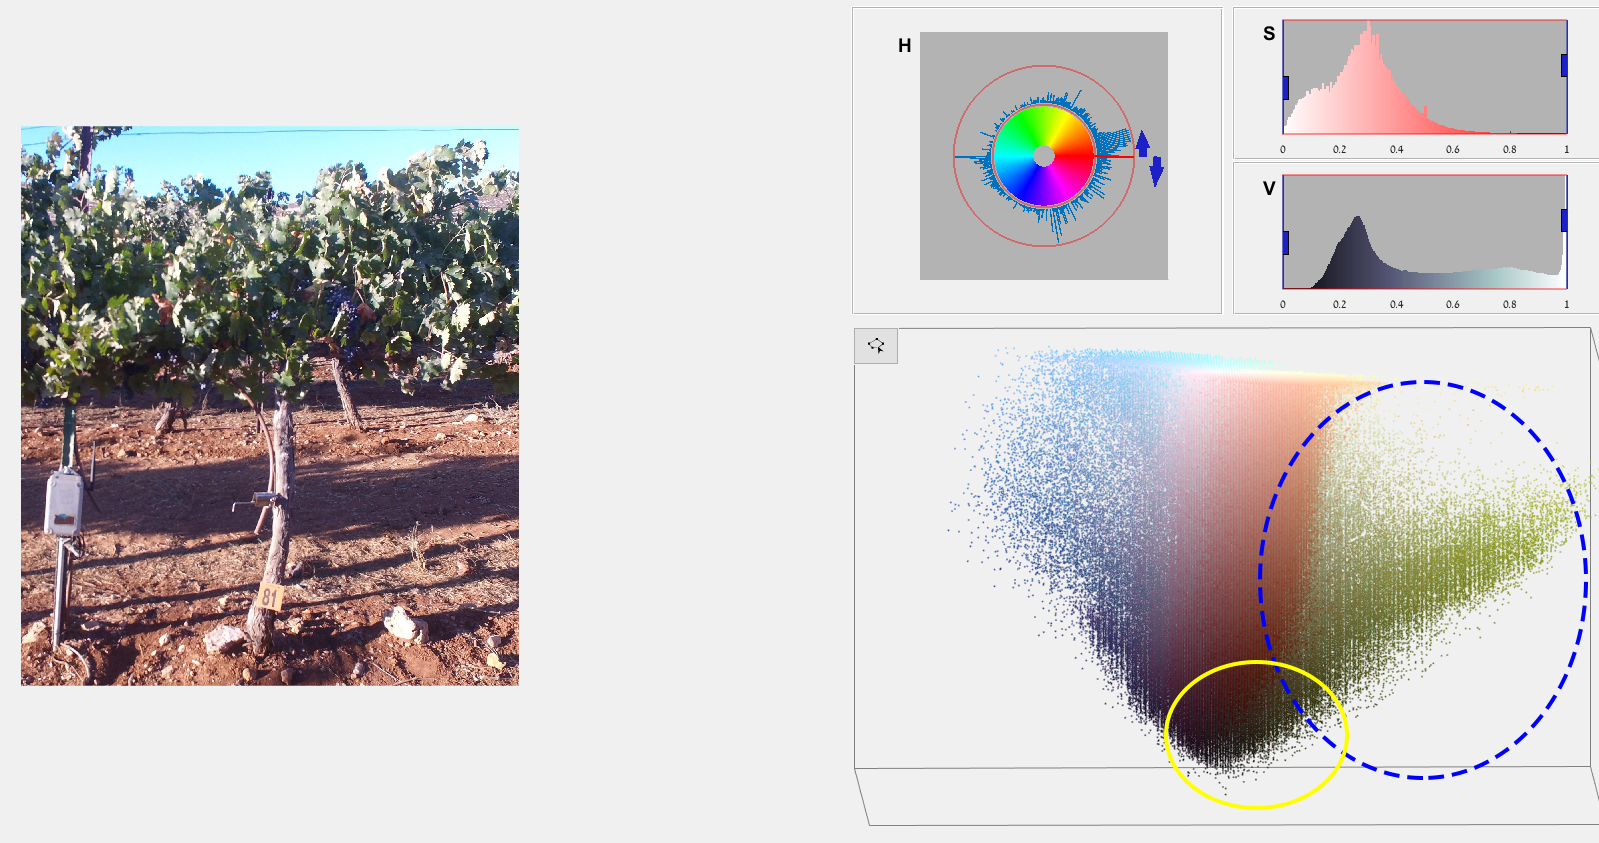
\includegraphics[width=0.9\columnwidth]{images/rgb2hsv.png} \par
    \caption{RGB to HSV}
    \label{fig:rgb2hsv}
\end{figure}

In the blue circle is the area that detected leaves, but in the yellow circle more leaves are hidden which are difficult to identify and need to calculate from the image.

\section{Research Methods}

\begin{enumerate}

\item image processing

\item Filtering

\item Algorithem

\item Data organization

\end{enumerate}


